% 封面装饰：二项分布 B(40, 1/2) 的直方图与正态密度曲线（de Moivre–Laplace）
\newcommand{\coveremblem}{%
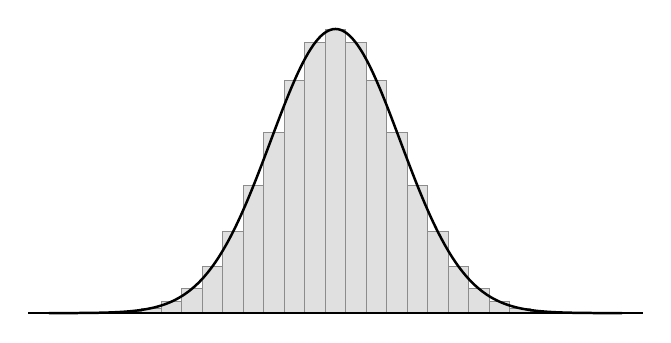
\begin{tikzpicture}[x=0.26cm,y=0.26cm]
  \pgfmathsetmacro{\s}{sqrt(10)}
  \foreach \k in {8,...,32}{
    \pgfmathsetmacro{\h}{110*exp(-(\k-20)^2/20)/(\s*sqrt(2*pi))}
    \fill[black!12] (\k-0.5,0) rectangle (\k+0.5,\h);
    \draw[black!45,line width=0.3pt] (\k-0.5,0) rectangle (\k+0.5,\h);
  }
  \draw[line width=0.9pt,domain=6:34,samples=120,smooth]
    plot (\x,{110*exp(-(\x-20)^2/20)/(\s*sqrt(2*pi))});
  \draw[line width=0.5pt] (5,0) -- (35,0);
\end{tikzpicture}}
